% =============================================================================
% ch03_sensors.tex — Chapter 3: Sensor Modalities | Biomimetic Navigator
% =============================================================================

\selectlanguage{hebrew}
\section{מודאליות החישנים: \en{LiDAR}, סונאר ו-\en{Vision-AI}}
\label{sec:sensors}

\subsection{מבוא להיתוך חיישנים רב-מודאלי}
כדי להשיג ניווט אוטונומי חסין (\en{robust}), המערכת שלנו משלבת שלושה סוגי חיישנים הפועלים בעקרונות פיזיקליים שונים. שילוב זה מאפשר התגברות על מגבלות אינדיבידואליות של כל חיישן, כגון רגישות לתנאי תאורה בראייה ממוחשבת או החזרות מראה (\en{specular reflections}) בסונאר.

\subsection{חיישן ה-\en{LiDAR}: גילוי ומדידת מרחק בלייזר}
חיישן ה-\en{LiDAR} מספק ענן נקודות (\en{point cloud}) ברזולוציה גבוהה. הוא פועל באמצעות מדידת זמן הטיסה (\en{ToF — Time of Flight}) של פולסי לייזר. מודל הרעש של ה-\en{LiDAR} מיוצג לרוב כהתפלגות גאוסיאנית:
\begin{equation}
    z_{\text{LiDAR}} = d + \eta_L, \quad \eta_L \sim \mathcal{N}(0, \sigma_L^2)
    \label{eq:lidar_noise}
\end{equation}
כאשר $\sigma_L$ הוא סטיית התקן האופיינית (לרוב בטווח של 2–5 ס"מ במערכות \en{MEMS LiDAR} מודרניות).

\subsection{מערך סונאר אולטרה-סוני \en{MEMS}}
בהשראת העטלף, אנו משתמשים במערך של חיישני סונאר. היתרון המרכזי של הסונאר הוא יכולתו לפעול בתנאי אבק, עשן או חשיכה מוחלטת שבהם חיישנים אופטיים עלולים להיכשל. המערכת משתמשת בעיבוד \en{Range-Doppler} כדי לחלץ את המרחק והמהירות היחסית של המכשולים.

\begin{figure}[H]
    \centering
    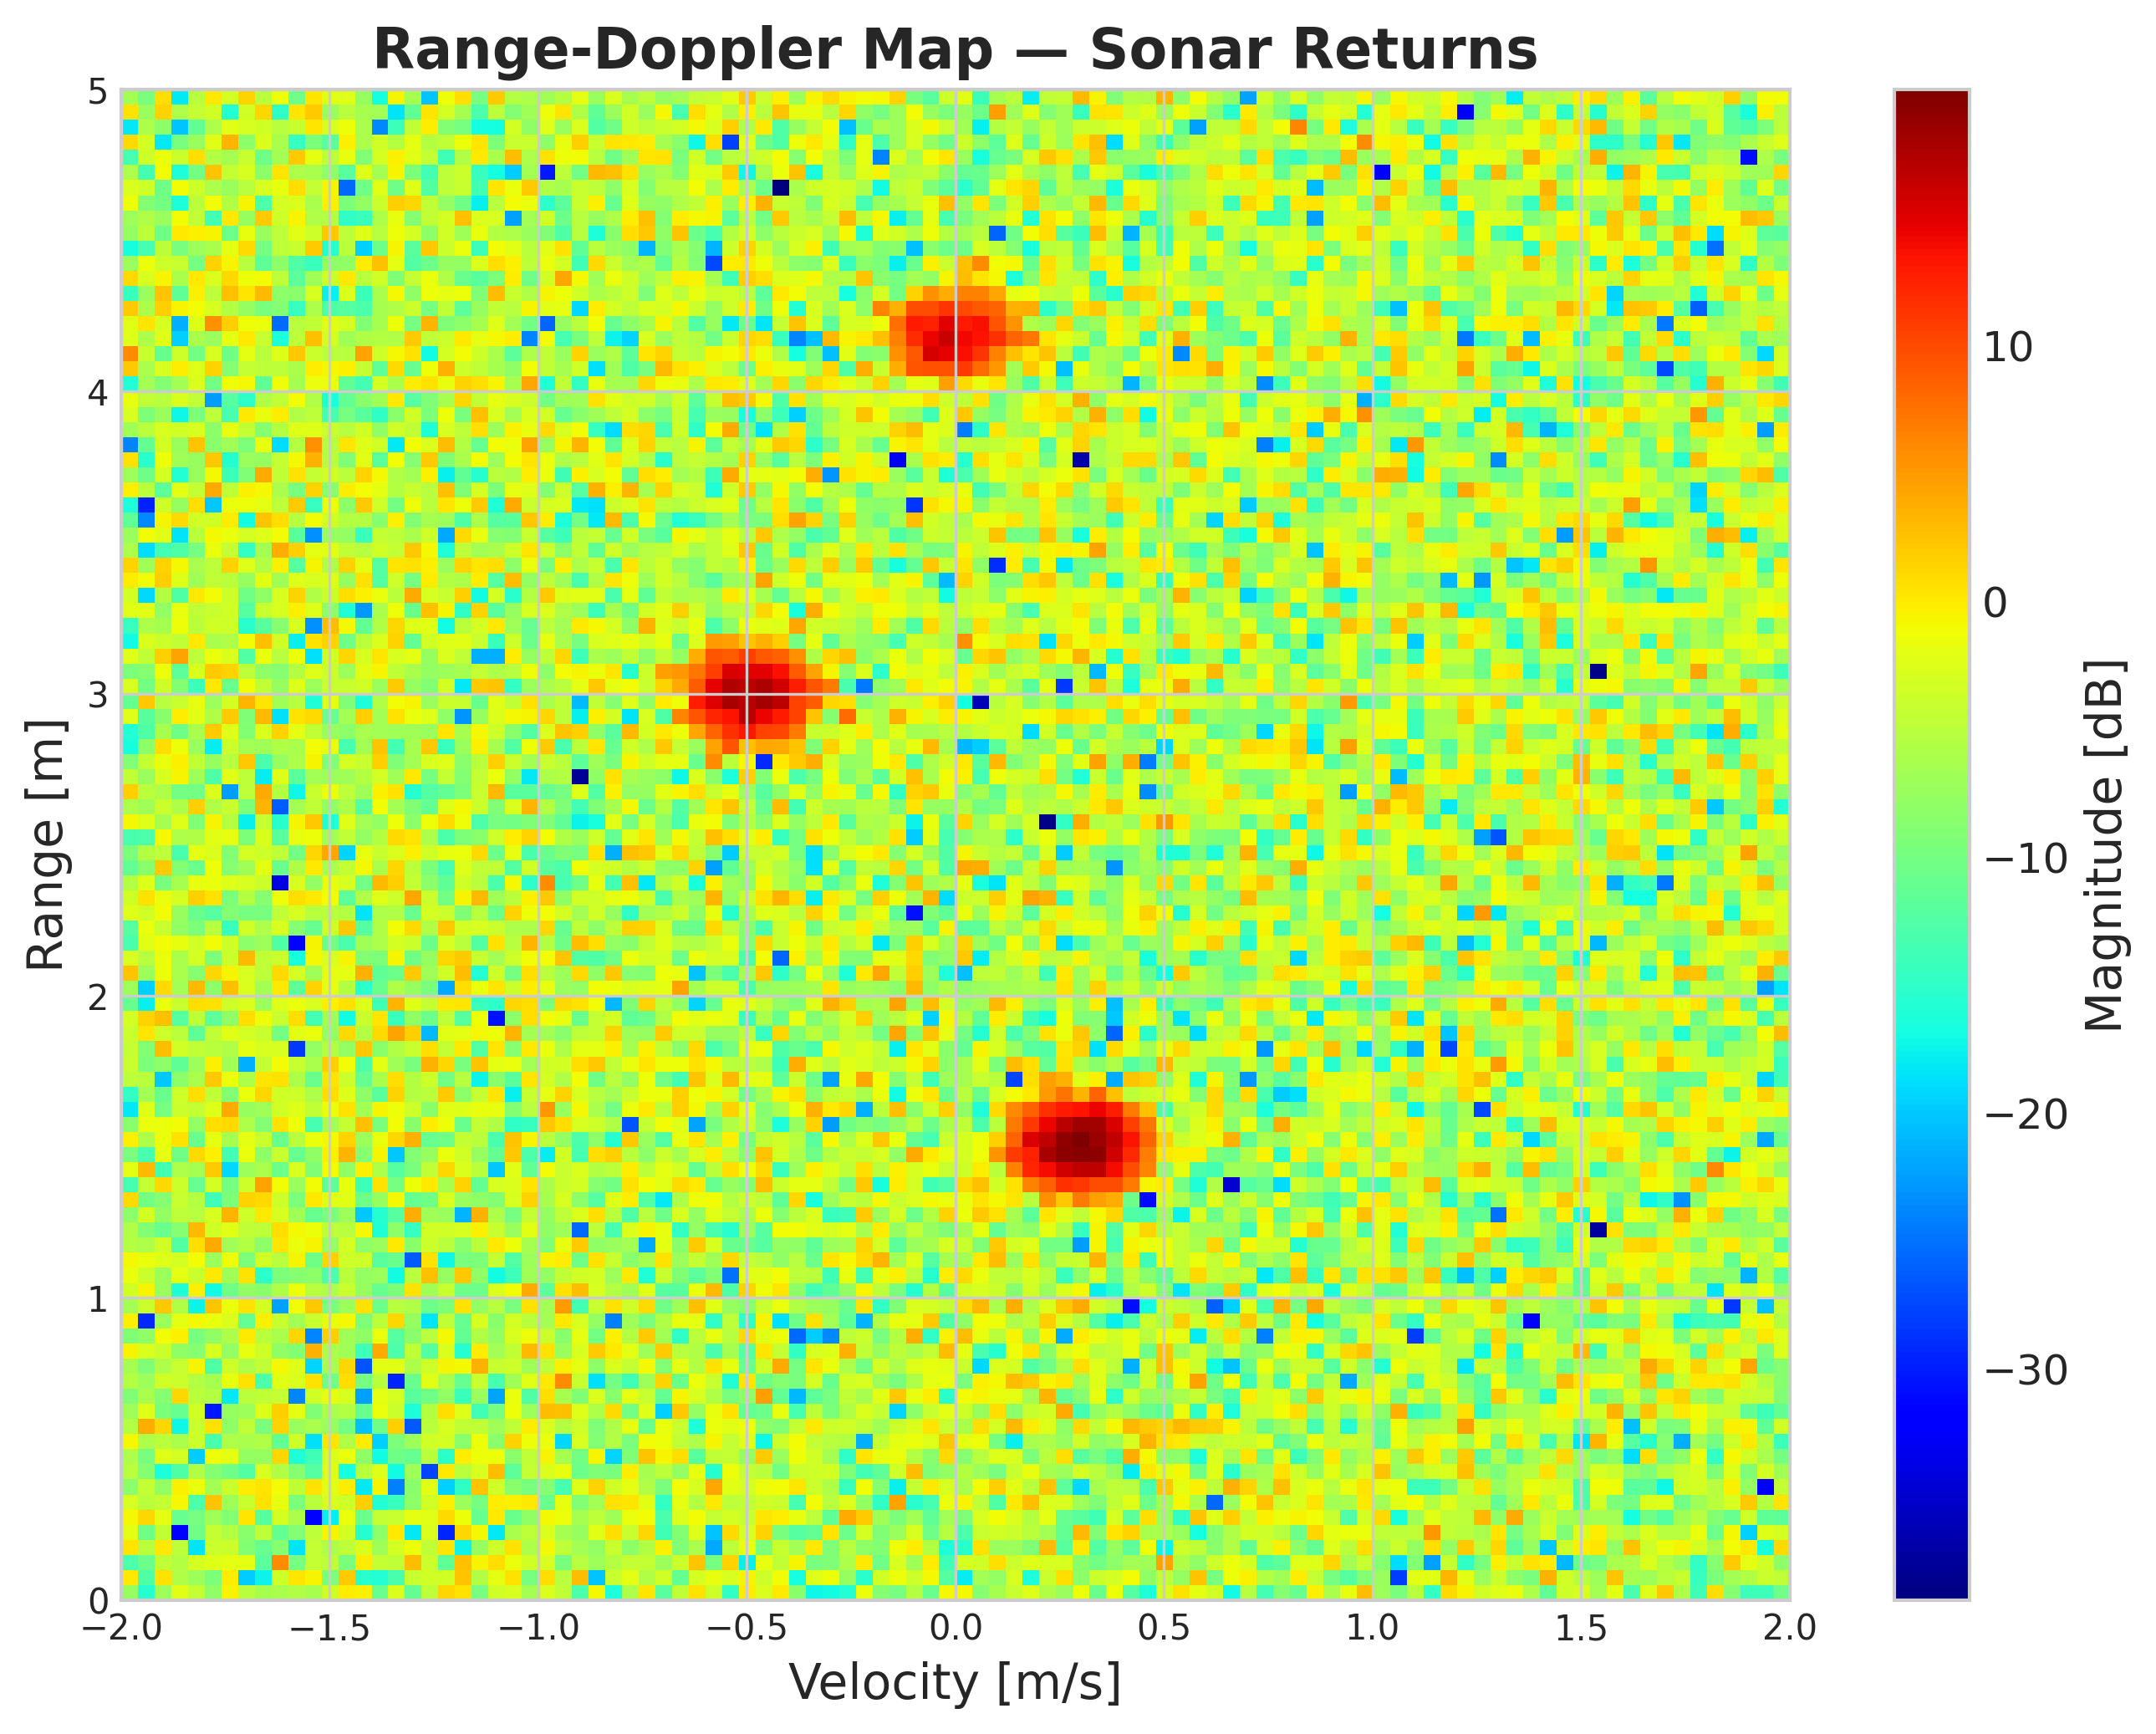
\includegraphics[width=0.8\columnwidth]{figures/fig_range_doppler.png}
    \caption{מפת טווח-דופלר המופקת מעיבוד אותות הסונאר. הנקודות הבהירות מסמנות עצמים מזוהים במרחב.}
    \label{fig:range_doppler}
\end{figure}

\subsection{ראייה ממוחשבת: \en{Vision-AI} לאמידת עומק}
המערכת משתמשת במודלי \en{Foundation} כגון \en{Depth Anything V2} כדי להפיק מפת עומק מתמונה בודדת (\en{monocular depth estimation}). מודלים אלו, המבוססים על ארכיטקטורות \en{Transformer}, מציגים יכולת הכללה (\en{generalization}) יוצאת דופן בסביבות חדשות. \cite{AnthropicClaude}

\begin{table}[H]
\centering
\begin{tabular}{lccc}
\toprule
מאפיין & \en{LiDAR} & סונאר & \en{Vision-AI} \\
\midrule
רזולוציה & גבוהה & נמוכה & בינונית \\
טווח פעולה & 0.1–100 מ' & 0.05–5 מ' & תלוי עדשה \\
חסינות לחשיכה & גבוהה & גבוהה מאוד & נמוכה \\
צריכת הספק & בינונית & נמוכה & גבוהה (חישוב) \\
\bottomrule
\end{tabular}
\caption{השוואת מאפייני החיישנים השונים במערכת ה-\en{NavigatorCrew}.}
\label{tab:sensor_comparison}
\end{table}

\subsection{תרשים זרימה של צינור החישה}
איור \ref{fig:sensor_modalities} מציג את אופן זרימת המידע מהחיישנים הגולמיים ועד ליצירת ייצוג הסביבה המאוחד.

\begin{figure}[H]
    \centering
    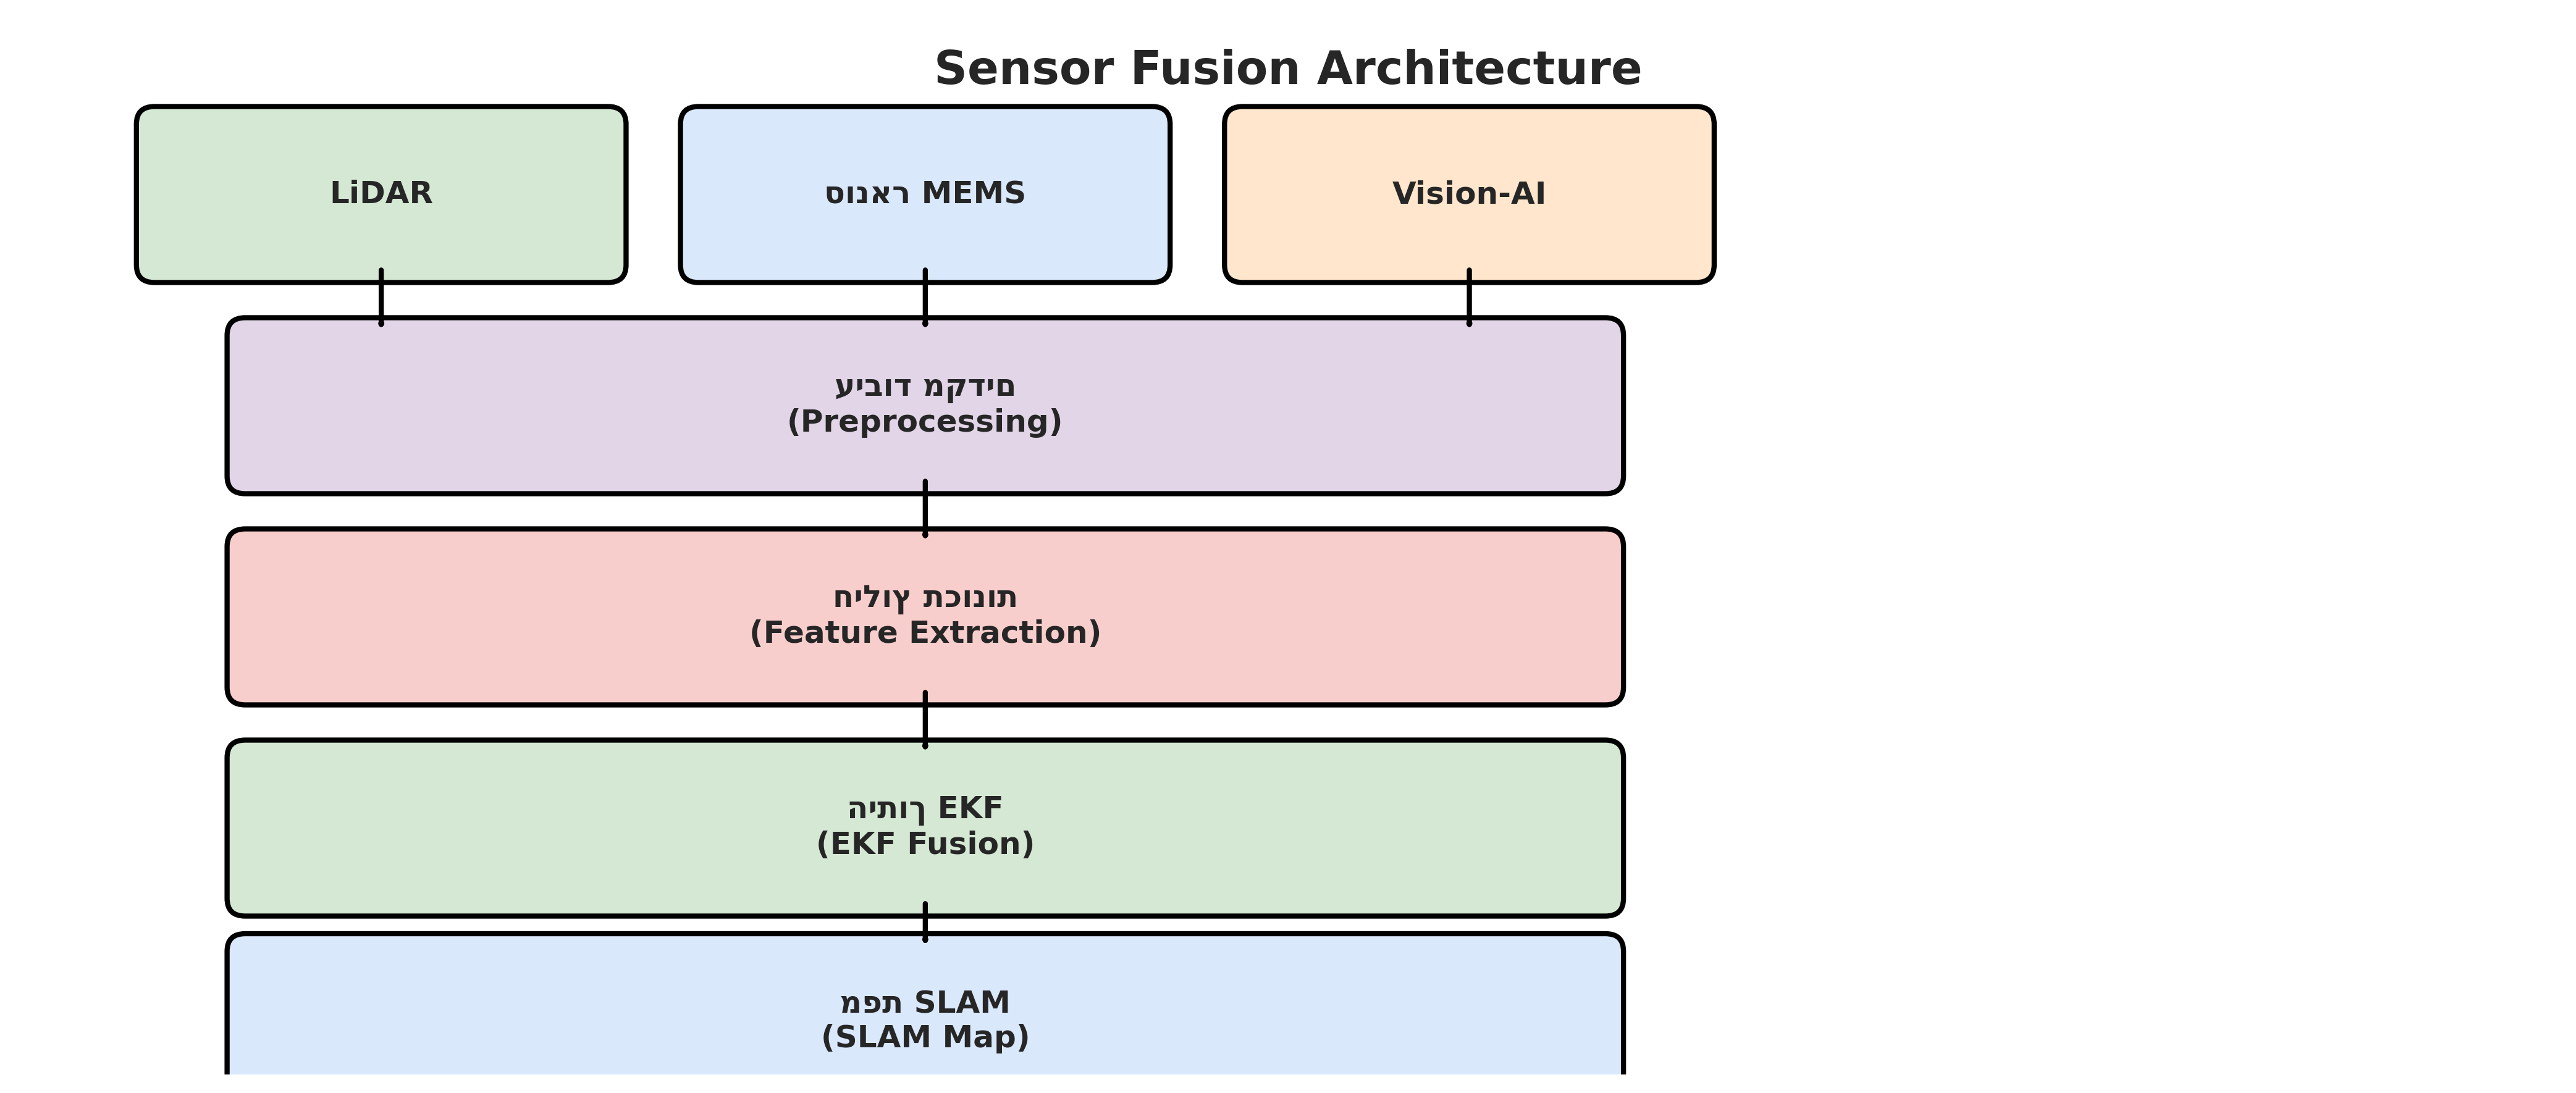
\includegraphics[width=0.9\columnwidth]{figures/fig_sensor_modalities.png}
    \caption{תרשים בלוקים של ארכיטקטורת החישה הרב-מודאלית.}
    \label{fig:sensor_modalities}
\end{figure}
